The picture below shows the networks of the first two test cases of the first example; tiles are labeled with their input values.

\begin{center}
  \def \htmlPixelsInCm {45}
  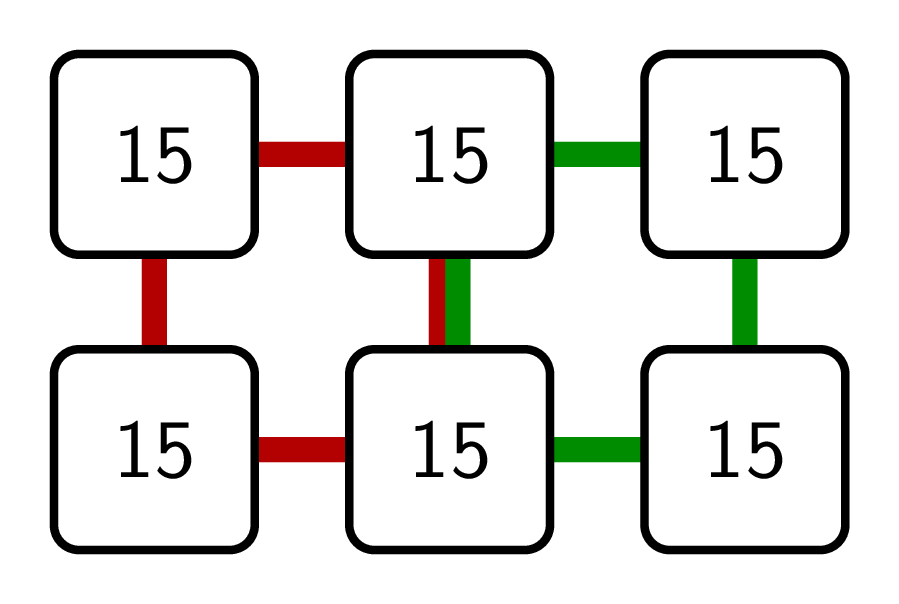
\includegraphics[width=8cm]{loops1.png} \\
  \small{First test case: every junction opens in all four directions; the two highlighted squares are one choice of independent loops --- they share the middle connection, yet two cuts are needed to break them both.}
\end{center}

\begin{center}
  \def \htmlPixelsInCm {45}
  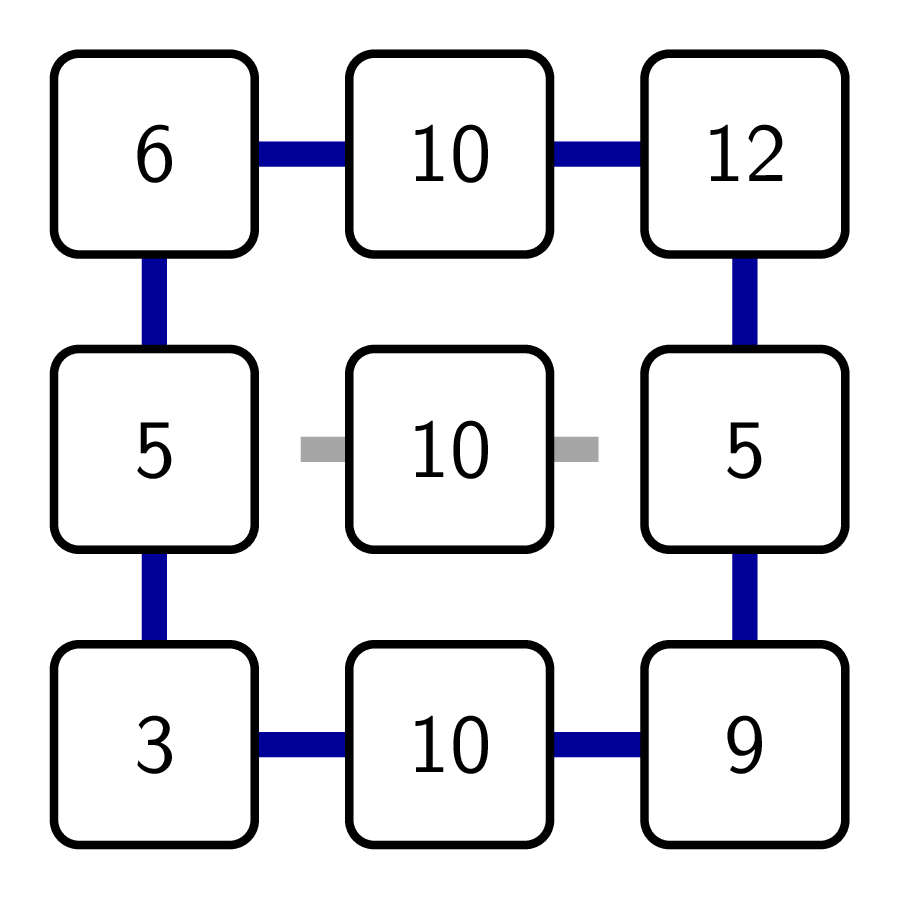
\includegraphics[width=8cm]{loops2.png} \\
  \small{Second test case: one single loop around the center; the center junction opens to the left and to the right, but nobody answers, so it is isolated.}
\end{center}

In the first test case every tile holds a $4$-opening junction, and two loops exist initially --- for example, the left and the right unit squares. The first impact destroys tile $(1,1)$, breaking the left square, so only one loop (the right square) remains. The second impact destroys tile $(1,2)$ and breaks that loop as well, and the third impact changes nothing. Hence the answers are $1, 0, 0$.

In the second test case eight junctions form a single loop around the center. The center tile $10$ opens to the left and to the right, but none of its neighbours opens back, so it is connected to nothing. The first impact destroys this isolated junction and the loop survives --- the answer is $1$. The second impact destroys tile $(1,2)$, cutting the ring into a path, so the answer becomes $0$.

In the third test case no two adjacent junctions ever face each other: tile $5$ does not open to the right and tile $6$ does not open to the left. There is not a single connection in the network, let alone a loop.

The fourth test case of the first example has $q = 0$, so the expected output for it is an empty line.

In the second example the network initially has two independent loops --- one around the left $3 \times 3$ block and one around the right $2 \times 3$ block --- plus one isolated junction. The first impact removes the isolated junction (answers start with $2$), the second and third impacts break the left and the right loop respectively, and the remaining impacts only shorten paths: $2, 1, 0, 0, 0, 0$.
